\documentclass[11pt,a4paper]{article}
\usepackage[margin=19mm,headheight=15pt]{geometry}
\usepackage[T1]{fontenc}
\usepackage{lmodern,microtype}
\usepackage{amsmath,booktabs,tabularx,array,enumitem}
\usepackage{xcolor,tikz,fancyhdr,titlesec,listings,hyperref}
\usetikzlibrary{arrows.meta,positioning,calc}
\definecolor{accent}{HTML}{244C3A}
\definecolor{wash}{HTML}{F1F5F0}
\definecolor{muted}{HTML}{59645E}
\hypersetup{colorlinks=true,urlcolor=accent,linkcolor=accent,pdftitle={PhotonicsAI Homework 3: Hardware in the Loop},pdfauthor={Aren Ananyan; David Sargsyan; Andranik Arakelyan; Yerem Bareghamyan}}
\setlength{\parindent}{0pt}
\setlength{\parskip}{5pt}
\setlength{\emergencystretch}{2em}
\setlist[itemize]{leftmargin=16pt,itemsep=2pt,topsep=3pt}
\titleformat{\section}{\large\bfseries\color{accent}}{\thesection}{0.6em}{}
\titleformat{\subsection}{\normalsize\bfseries}{\thesubsection}{0.6em}{}
\titlespacing*{\section}{0pt}{9pt}{5pt}
\titlespacing*{\subsection}{0pt}{7pt}{3pt}
\pagestyle{fancy}\fancyhf{}
\fancyhead[L]{\small\color{muted}PhotonicsAI \;|\; Homework 3}
\fancyhead[R]{\small\color{muted}Hardware in the Loop}
\fancyfoot[L]{\small Team submission \;\textbullet\; 18 October 2026}
\fancyfoot[R]{\small\thepage}
\renewcommand{\headrulewidth}{0.3pt}
\newcommand{\code}[1]{\texttt{\small #1}}
\newcommand{\note}[1]{\par\smallskip\noindent\fcolorbox{accent}{wash}{\parbox{\dimexpr\linewidth-2\fboxsep-2\fboxrule\relax}{#1}}\par\smallskip}
\newcommand{\repo}{https://github.com/Arenananyan/photonicsai-homework-3}
\newcommand{\evidence}[2]{\href{https://github.com/Arenananyan/photonicsai-homework-3/tree/main/docs/evidence/#1}{#2}}
\lstset{basicstyle=\ttfamily\footnotesize,breaklines=true,columns=fullflexible,keepspaces=true,frame=single,rulecolor=\color{accent},backgroundcolor=\color{wash},aboveskip=5pt,belowskip=5pt}
\tikzset{box/.style={draw=accent,rounded corners=3pt,fill=wash,align=center,font=\small,minimum height=9mm},arrow/.style={-{Stealth[length=2mm]},draw=accent,thick},lane/.style={draw=muted!55,dashed}}
\begin{document}
\begin{center}
{\small\color{muted}AI-DRIVEN SCIENCE AND AUTONOMOUS LABORATORIES}\par
{\LARGE\bfseries\color{accent}Homework 3}\par
{\Large Hardware in the Loop}\par\medskip
{\normalsize Aren Ananyan \;\textbullet\; David Sargsyan}\par
{\normalsize Andranik Arakelyan \;\textbullet\; Yerem Bareghamyan}\par
{\small 18 October 2026}
\end{center}

\section{System and demonstrated scope}
We adapt the four-role laboratory workflow into a LangGraph application with
MCP instrument tools and a human stop before motion. The executor proposes an
instrument operation, the graph validates and dispatches it, and the measured
response returns to shared dialogue before the next decision.

\note{\textbf{Evidence scope.} The complete recorded run uses a scripted decision
model and a mock printer. It demonstrates actual LangGraph execution, stdio MCP
communication, human approval and post-execution measurement. A separate earlier
run demonstrates a live Groq status read against the mock printer. A successful
live-LLM movement run on the physical printer is not established by this submission.}

\textbf{Code, evidence and videos:}
\href{\repo}{github.com/Arenananyan/photonicsai-homework-3}

\section{Architecture}
\begin{center}
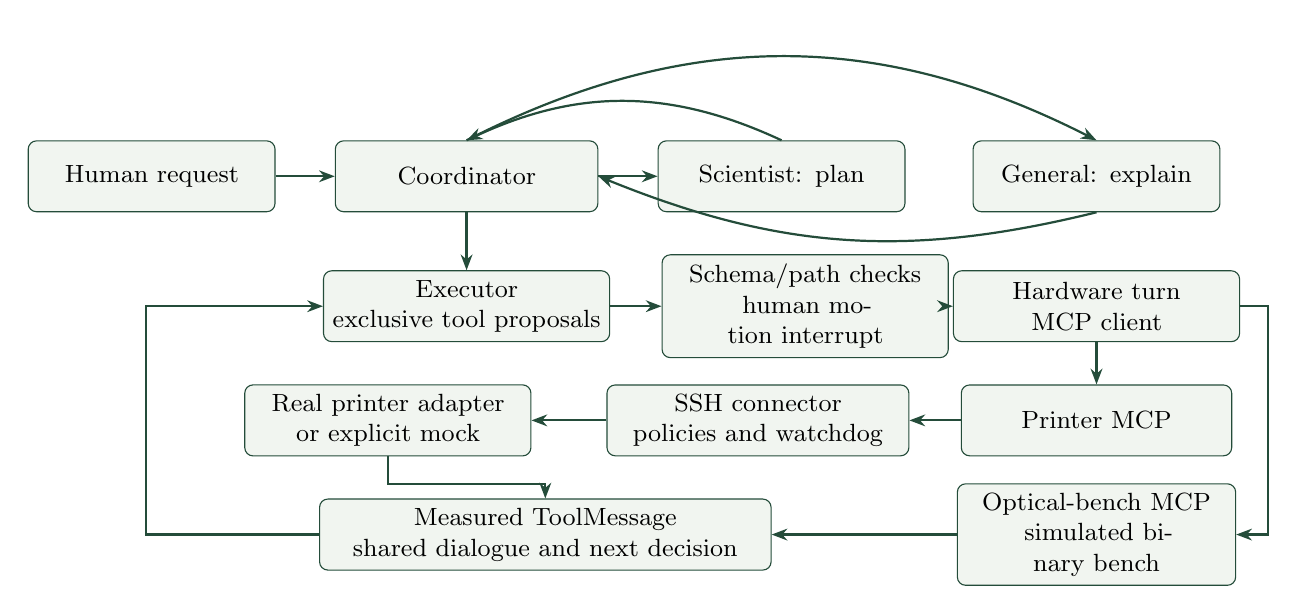
\begin{tikzpicture}[node distance=7mm]
\node[box,text width=29mm] (human) at (0,0) {Human request};
\node[box,text width=31mm] (coord) at (4,0) {Coordinator};
\node[box,text width=29mm] (science) at (8,0) {Scientist: plan};
\node[box,text width=29mm] (general) at (12,0) {General: explain};
\node[box,text width=34mm] (exec) at (4,-1.65) {Executor\\exclusive tool proposals};
\node[box,text width=34mm] (guard) at (8.3,-1.65) {Schema/path checks\\human motion interrupt};
\node[box,text width=34mm] (turn) at (12,-1.65) {Hardware turn\\MCP client};
\node[box,text width=32mm] (pmcp) at (12,-3.1) {Printer MCP};
\node[box,text width=36mm] (connector) at (7.7,-3.1) {SSH connector\\policies and watchdog};
\node[box,text width=34mm] (printer) at (3,-3.1) {Real printer adapter\\or explicit mock};
\node[box,text width=33mm] (bench) at (12,-4.55) {Optical-bench MCP\\simulated binary bench};
\node[box,text width=55mm] (result) at (5,-4.55) {Measured ToolMessage\\shared dialogue and next decision};
\draw[arrow] (human)--(coord);
\draw[arrow] (coord)--(science);
\draw[arrow] (science.north) to[bend right=25] (coord.north);
\draw[arrow] (coord.north) to[bend left=27] (general.north);
\draw[arrow] (general.south) to[bend left=18] (coord.east);
\draw[arrow] (coord)--(exec);
\draw[arrow] (exec)--(guard);
\draw[arrow] (guard)--(turn);
\draw[arrow] (turn)--(pmcp);
\draw[arrow] (pmcp)--(connector);
\draw[arrow] (connector)--(printer);
\draw[arrow] (turn.east) -- ++(0.35,0) |- (bench.east);
\draw[arrow] (printer.south) -- ++(0,-0.35) -| (result.north);
\draw[arrow] (bench)--(result);
\draw[arrow] (result.west) -- ++(-2.2,0) |- (exec.west);
\end{tikzpicture}
\end{center}
The roles retain their earlier responsibilities; their prompts and graph are
adapted for this standalone instrument task. The previous Silverbox training
executor is not imported unchanged. The Homework 2 bench remains a simulation.

\newpage
\section{Connector, MCP tools and decision loop}
\subsection{Instrument interface}
The target instrument is the team's 3-D printer, using its Klipper-compatible
controller software through an authenticated shared SSH session. The remote
watchdog connects to Klipper's Unix-domain API socket, \code{/tmp/klippy\_uds}.
It reads \code{objects/query} and submits validated motion using \code{gcode/script}.
JSON requests and responses are delimited by byte 0x03. The connector reads
reported XYZ, readiness, homed axes and travel bounds. The exact printer make and
model have not been independently documented in the supplied evidence.

The reused printer modules implement the client, policy checks, watchdog,
command handling and MCP server. The source manifest lists their filenames and
hashes; the original printer license is
included. Real mode uses the current operator-configured SSH host and control
socket; mock mode instantiates the simulated connector instead.

\subsection{Exposed operations}
\begin{tabularx}{\linewidth}{@{}p{43mm}X@{}}
\toprule
\textbf{MCP tool} & \textbf{Action or returned measurement}\\\midrule
\code{printer\_status} & Reads readiness, XYZ, homed axes and controller telemetry.\\
\code{preview\_sequence} & Validates relative XYZ steps; returns absolute waypoints, speed, bounds and an expiring token.\\
\code{preview\_position} & Previews an absolute target; host path checks still apply.\\
\code{execute\_sequence} & Executes one approved preview token. Reads/preview operations do not move the instrument.\\
\code{measure\_binary\_pattern} & Sets simulated on/off macropixels and returns optical measurements.\\\bottomrule
\end{tabularx}

\subsection{One agent holds the tools}
In live mode, only executor receives discovered MCP schemas. Groq returns a JSON
proposal such as \code{\{"tool":"printer\_status","arguments":\{\}\}}. The host
validates its tool name and arguments and converts it into an AIMessage tool call;
the hardware node then invokes MCP. The tool selection is model-generated in live
mode, while the recorded demonstration substitutes an explicitly scripted model.

Coordinator routes the shared dialogue; scientist supplies plans; general supplies
explanations. Each instrument response becomes a ToolMessage. Executor reads that
measurement on its following turn; after execution it must request a fresh status
before concluding. This separates a proposed action from a measured outcome.

\subsection{Motion and approval controls}
A valid path lifts vertically to $Z_c=\max(100,Z_{\rm start},Z_{\rm target})$ mm,
travels in XY at that height, then lowers if necessary. Zero-distance steps are
removed; simultaneous XYZ diagonals and low XY travel are rejected. Requested
speeds must be finite and at most 30 mm/s. Bounds and controller state are also
checked by the connector.

A LangGraph interrupt displays the actual preview. Approval must match its call ID
and live token. The host allows at most 110 seconds, within the MCP token's
120-second lifetime. A dispatch claim is written before execution; refusal,
expired tokens and uncertain outcomes do not trigger automatic movement retries.
Real motion additionally requires the operator's motion-enable setting.

\newpage
\section{Use case A: approved simulated movement}
\textbf{Recorded request:} ``Plan a simulated move to X110 Y110 Z100, preview it,
wait for approval, execute once and measure the final position.''

\textbf{Mode:} scripted model, mock printer, actual stdio MCP servers.
\textbf{Evidence:} \evidence{simulation-approved}{approved-run audit and dialogue}.

\begin{center}
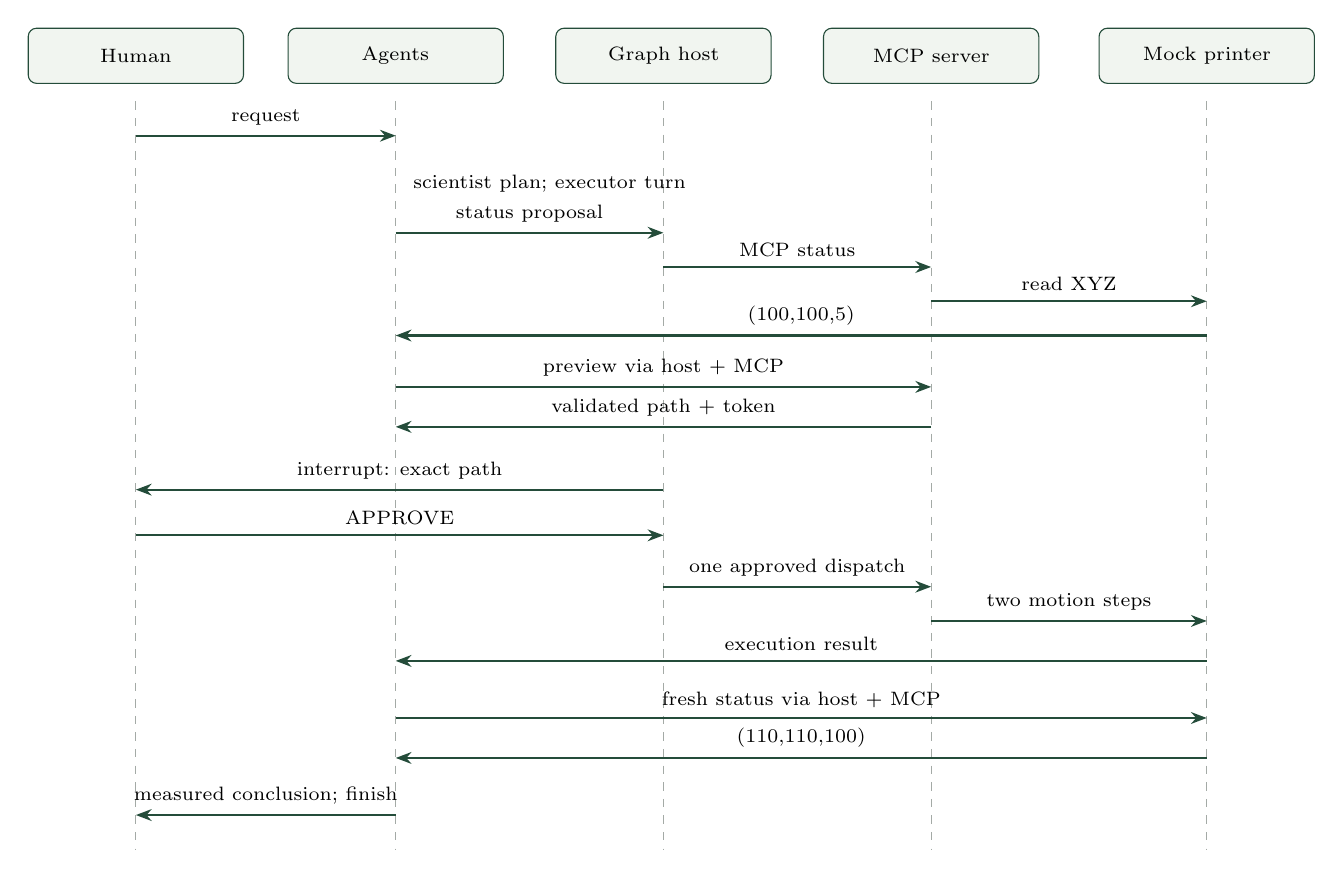
\begin{tikzpicture}[x=1cm,y=1.45cm,font=\scriptsize]
\foreach \x/\label in {0.4/Human,3.7/Agents,7.1/Graph host,10.5/MCP server,14/Mock printer}{
 \node[box,minimum height=7mm,text width=25mm,font=\scriptsize] at (\x,0) {\label};
 \draw[lane] (\x,-0.4)--(\x,-6.95);
}
\draw[arrow] (0.4,-0.7)--node[above]{request} (3.7,-0.7);
\node[anchor=west] at (3.8,-1.12) {scientist plan; executor turn};
\draw[arrow] (3.7,-1.55)--node[above]{status proposal} (7.1,-1.55);
\draw[arrow] (7.1,-1.85)--node[above]{MCP status} (10.5,-1.85);
\draw[arrow] (10.5,-2.15)--node[above]{read XYZ} (14,-2.15);
\draw[arrow] (14,-2.45)--node[above]{(100,100,5)} (3.7,-2.45);
\draw[arrow] (3.7,-2.9)--node[above]{preview via host + MCP} (10.5,-2.9);
\draw[arrow] (10.5,-3.25)--node[above]{validated path + token} (3.7,-3.25);
\draw[arrow] (7.1,-3.8)--node[above]{interrupt: exact path} (0.4,-3.8);
\draw[arrow] (0.4,-4.2)--node[above]{APPROVE} (7.1,-4.2);
\draw[arrow] (7.1,-4.65)--node[above]{one approved dispatch} (10.5,-4.65);
\draw[arrow] (10.5,-4.95)--node[above]{two motion steps} (14,-4.95);
\draw[arrow] (14,-5.3)--node[above]{execution result} (3.7,-5.3);
\draw[arrow] (3.7,-5.8)--node[above]{fresh status via host + MCP} (14,-5.8);
\draw[arrow] (14,-6.15)--node[above]{(110,110,100)} (3.7,-6.15);
\draw[arrow] (3.7,-6.65)--node[above]{measured conclusion; finish} (0.4,-6.65);
\end{tikzpicture}
\end{center}

\begin{tabularx}{\linewidth}{@{}p{28mm}rrrX@{}}\toprule
\textbf{Waypoint} & \textbf{X} & \textbf{Y} & \textbf{Z} & \textbf{Meaning (mm)}\\\midrule
Start &100&100&5&Initial mock status\\
Lift &100&100&100&Relative Z increase of 95\\
Target &110&110&100&Relative XY increase of (10,10)\\\bottomrule
\end{tabularx}

Both segments use 10 mm/s. The preview estimates 10.914 s of nominal travel;
this is a planner estimate, not a measured physical duration. The mock connector
returns two commands and reported position (110,110,100). A separate subsequent
status read returns the same XYZ. The final simulated residual is
$\lVert\mathbf p_{\rm measured}-\mathbf p_{\rm target}\rVert_2=0$ mm.

\note{The graph paused before execution. The audit contains a matching human
approval followed by exactly one execution request and then a new status request.
These observations establish the software loop in mock mode, not physical accuracy.}

\newpage
\section{Additional use cases and sequences}
\subsection{B. Refused simulated movement}
The recorded request asks scientist for one short plan, then executor to read
simulated status, preview a safe move to X110 Y110 Z100 at 10 mm/s, wait for host
approval, execute once and read status again. The operator instead declines.

\textbf{Observed calls:} \code{printer\_status} $\rightarrow$
\code{preview\_sequence}. There is no \code{execute\_sequence} call. The preview's
end coordinate is only a proposed destination, not evidence of movement.
\textbf{Evidence:} \evidence{simulation-declined}{refused-run audit and dialogue}.

\begin{center}
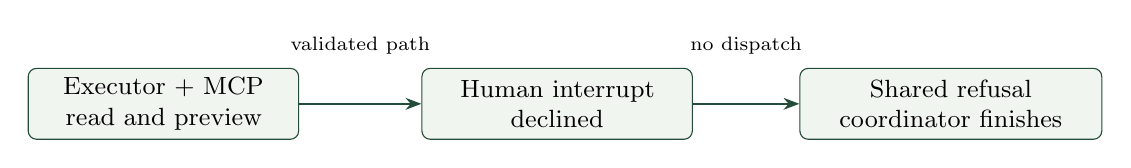
\begin{tikzpicture}[font=\small]
\node[box,text width=32mm] (a) at (0,0) {Executor + MCP\\read and preview};
\node[box,text width=32mm] (b) at (5,0) {Human interrupt\\declined};
\node[box,text width=36mm] (c) at (10,0) {Shared refusal\\coordinator finishes};
\draw[arrow] (a)--node[above=5mm,font=\scriptsize]{validated path}(b);
\draw[arrow] (b)--node[above=5mm,font=\scriptsize]{no dispatch}(c);
\end{tikzpicture}
\end{center}

\subsection{C. Binary optical-bench measurement}
The saved CLI request is ``Simulation verification'', executed with the explicit
scripted \code{bench} scenario. That scenario selects all 256 macropixels as on in
a $16\times16$ binary pattern. Its MCP call is
\code{measure\_binary\_pattern}, with indices 0 through 255. The simulator is seeded
with 42.

\begin{tabularx}{\linewidth}{@{}Xr@{}}\toprule
\textbf{Returned simulated quantity} & \textbf{Value}\\\midrule
On macropixels &256\\
Enhancement &1.542110\\
Target mean &1.473747\\
Background mean &0.955669\\\bottomrule
\end{tabularx}
\textbf{Sequence:} coordinator $\rightarrow$ scientist $\rightarrow$ executor
$\rightarrow$ bench MCP $\rightarrow$ simulated measurement $\rightarrow$
executor conclusion $\rightarrow$ coordinator finish.
This is a measurement example, not an optimized focusing experiment.
\textbf{Evidence:} \evidence{simulated-optical-bench}{bench audit and dialogue}.

\subsection{D. Live Groq status read, mock printer}
\textbf{Recorded request:} ``Read printer status only, explicitly label simulated
readings, explain measured XYZ, finish without movement.''

An earlier live Groq run selects \code{printer\_status}. The MCP response reports
\code{simulated: true} and XYZ (100,100,5); no motion tool is dispatched. The
following model turn reads and explains the response before coordinator finishes.
\textbf{Sequence:} coordinator $\rightarrow$ executor model decision $\rightarrow$
MCP status $\rightarrow$ mock telemetry $\rightarrow$ executor model explanation
$\rightarrow$ coordinator finish.
\textbf{Evidence:} \evidence{live-groq-mock-status}{live-model read-only transcript}.

This earlier run supports a limited live model/tool interaction. It does not
validate the current complete live movement workflow, which encountered repeated
planning and Groq rate-limit failures during subsequent attempts.

\newpage
\section{Validation, videos and reproducibility}
\subsection{Software checks}
Fifteen tests passed on 18 October 2026, together with dependency consistency and
Ruff lint/format checks. MCP integration tests start actual stdio servers; model
responses are scripted or mocked in automated tests.
\begin{itemize}
\item Approval refusal, wrong IDs, expiry and unknown tokens block dispatch.
\item Single-use claims and uncertain execution prevent automatic repetition.
\item A successful execution requires a fresh status before another action or conclusion.
\item Path geometry, finite speeds, zero-distance steps and tool-loop limits are checked.
\item Clarification resumes the same dialogue; only executor receives tool schemas.
\item The compact JSON proposal adapter is tested through MCP and a human pause.
\end{itemize}
Passing tests do not establish live-LLM task reliability or physical hardware success.

\subsection{Available videos}
Both files are in the repository's \href{\repo/tree/main/videos}{videos directory}.
\begin{itemize}
\item \textbf{Screen Recording 2026-10-18 at 00.07.16.mov:} the supplied recording
of the scripted LangGraph/MCP simulation. The matching transcript is
\evidence{simulation-approved}{the approved-run evidence directory}. It shows the preview, human stop,
approval, mock execution and post-execution read.
\item \textbf{IMG\_9999.MOV:} existing operator-supplied footage intended as
physical-printer context. Its exact capture date, project version and contents
have not been independently verified for this report. It is not evidence that
the new graph controlled that hardware.
\end{itemize}

\subsection{Reproduce the recorded software loop}
Install Python 3.12+ and the pinned requirements, then run from the repository root:
\begin{lstlisting}
python3 -m venv .venv
.venv/bin/python -m pip install -r requirements.lock.txt
.venv/bin/python -m hw3.cli \
  "Plan a simulated move to X110 Y110 Z100, preview it, wait for approval, execute once and measure the final position." \
  --mode mock --demo --scenario move
\end{lstlisting}
Type \code{APPROVE} only after reviewing the displayed path; any other reply
declines. New runs create local \code{results/} records. Tests run with
\code{.venv/bin/python -m unittest discover -s tests -v}. Live mode omits
\code{--demo} and requires a locally configured Groq key; real mode additionally
requires an authenticated SSH session and explicit operator motion enablement.

\subsection{Requirement coverage and remaining gap}
The repository supplies the connector and MCP implementation, executor-only model
tool proposals, a hardware turn with measured results, diagrams and multiple
recorded software use cases. The complete accepted run is simulated with scripted
decisions. The assignment's real-instrument, model-driven end-to-end demonstration
remains incomplete: exact hardware identity and a successful new-graph run on that
instrument are still required. The existing real-printer footage and earlier
live-model mock-status read should be evaluated only within their stated scope.

\textbf{Source code and supporting material:}
\href{\repo}{github.com/Arenananyan/photonicsai-homework-3}.
The editable source of this report is \code{docs/report/main.tex}.
\end{document}
